\chapter{Materiali e metodi\ok \ok \ok}

\section{Il Dataset: Severstal steel defect detection \ok}

L'acciaio è uno dei materiali più comunemente utilizzati in tutto il mondo, e la sua produzione e il suo costo sono in continua crescita, come è possibile vedere
dal report rilasciato nel 2022 dalla World Steel Association \cite{worldsteelreport2021}, un'organizzazione \textit{no-profit} impegnata 
nello sviluppo di questo settore.
Tale documento mostra come la produzione di acciaio sia stata in continua crescita negli ultimi 70 anni, e come la produzione mondiale di acciaio
abbia raggiunto le 1.95 miliardi di tonnellate nel 2021 in crescita del 3.8\% rispetto al 2020, e si prevede che questa crescita continui nei prossimi anni, 
salvo momentanee battute d'arresto dovute a crisi economiche o pandemie.
La sua versatilità e la sua resistenza lo rendono un materiale molto utilizzato in diversi settori, come l'edilizia, l'automotive, l'industria elettronica, l'industria aerospaziale, ecc.
Per produzioni su larga scala di acciaio come di altri materiali o prodotti, è necessario che il materiale sia di qualità, e che non contenga difetti,
ma è difficile per gli operatori umani rilevare difetti come graffi, crepe, ecc. con elevata affidabilità, per tale ragione 
è necessario adottare sistemi automatizzati che siano in grado di rilevare difetti in modo affidabile e veloce.

L'automatizzazione del controllo qualità è stata la scelta fatta da Severstal, una delle principali aziende produttrici di acciaio in Russia, che produce circa 10 milioni di tonnellate di acciaio 
all'anno. Severstal ha messo a disposizione \textbf{Severstal steel defect detection dataset} nel 2019 per permettere a chiunque di testarvi le proprie idee, 
sperando di riuscire ad aumentare l'affidabilità del proprio sistema di rilevazione difetti sfruttando la comunita di Kaggle.
Il dataset è disponibile al seguente link: \url{https://www.kaggle.com/c/severstal-steel-defect-detection/data}.

Questo dataset è diviso in 2 parti, training e test set, ma per il test set non sono stati rilasciati i ground truth, quindi non è possibile testare
il modello sul test set originale e verranno dunque utilizzati solo i dati del training set, i quali verranno suddivisi in training e test set.
Il training set originale  è composto da 12568 immagini, che verranno divise in un 50\% per il nuovo training set e 50\% per il nuovo test set, 
quindi un totale di 6284 immagini per il training set e 6284 immagini per il test set. 
Questo numero è stato scelto in modo da garantire un numero minimo di immagini per effettuare l'addestramento del modello, in quanto 
lo scopo non è addestrare un buon modello ma valutare l'efficacia del metodo per dataset di piccole dimensioni. 

il training set è stato poi utilizzato per il training del generatore di difetti sintetici, mentre il test set per valutare la qualità dei dati generati
tramite FID score.

\subsection{Distribuzione del dataset}
\begin{comment}
    Cosa posso scrivere in questa sezione?
    - descrizione del dataset
    - descrizione delle immagini
    - descrizione delle classi
    - descrizione della distribuzione delle classi
\end{comment}
In questa sezione viene presentata un'analisi tecnica della distribuzione del dataset, considerando il numero di immagini,
numero e distribuzione dei poligoni in esse, per comprendere nel dettaglio il dataset e la sua composizione.

Il Severstal dataset è composto come già detto da 12568 immagini di lastre di acciaio con risoluzione 256x1600,
di queste immagini abbiamo 6666 immagini con difetti, e 5902 immagini senza difetti. Il severstal dataset presenta 4 classi di difetti,
le quali purtroppo, come spesso accade nei dataset provenienti da casi reali, non sono bilanciate, infatti abbiamo:

% tabella che riassume i valori sopra citati
\begin{table}[H]
    \centering
    \begin{tabular}{|c|c|c|c|c|}
    \hline
            & \textbf{Classe 1} & \textbf{Classe 2} & \textbf{Classe 3} & \textbf{Classe 4} \\
    \hline
    \textbf{Numero di poligoni} & 3082 & 321 & 14622 & 1902 \\
    \hline
    \end{tabular}
    \caption{Distribuzione delle immagini per classe.}
    \label{tab:sd_polygons_distribution}
\end{table}


    \begin{figure}[H]
        \centering
        \begin{tabular}{cc}
            % first row
            \subfloat[Distribuzione delle immagini con e senza difetti.]{
                \label{fig:sd_images_distribution}
                \centering
                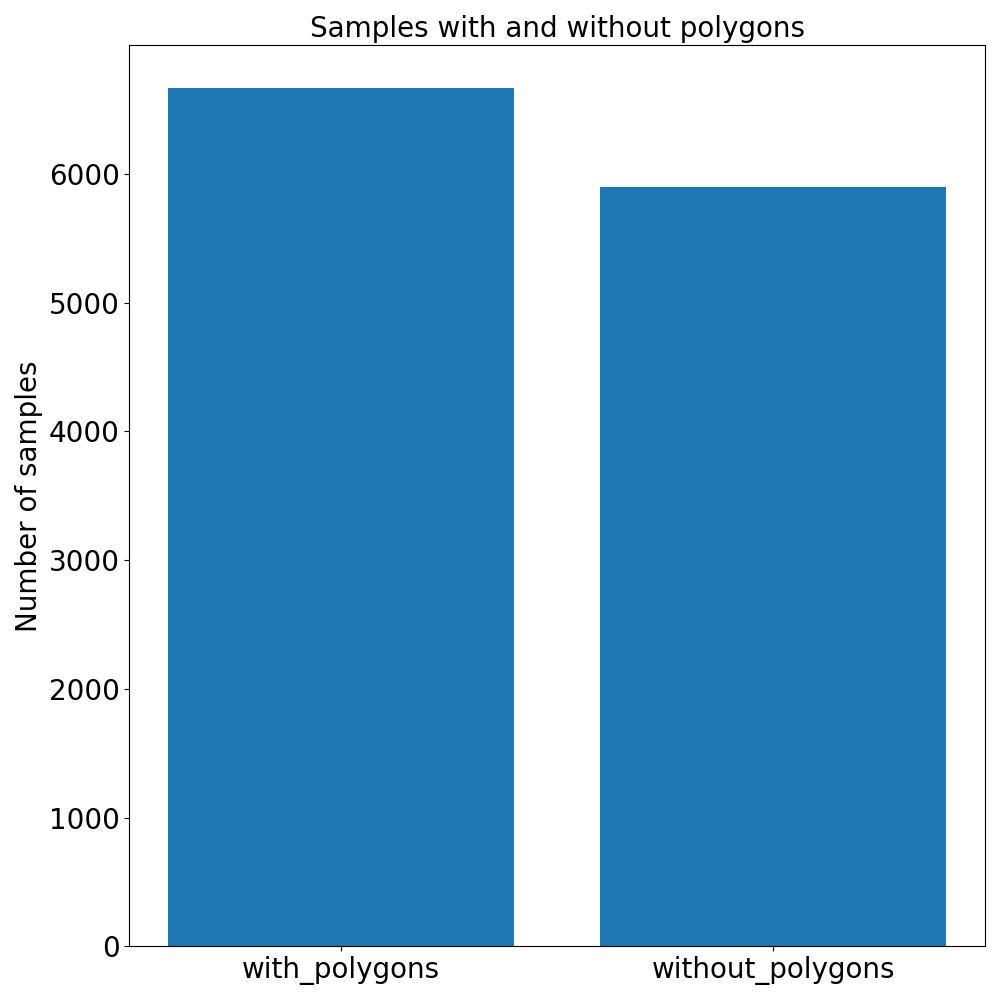
\includegraphics[width=0.45\textwidth]{imgs/Severstal/raw_dataset/samples_with_and_without_polygons_histogram.png}
            }  &
            \subfloat[Distribuzione dei poligoni per classe.]{
                \label{fig:sd_polygons_distribution}
                \centering
                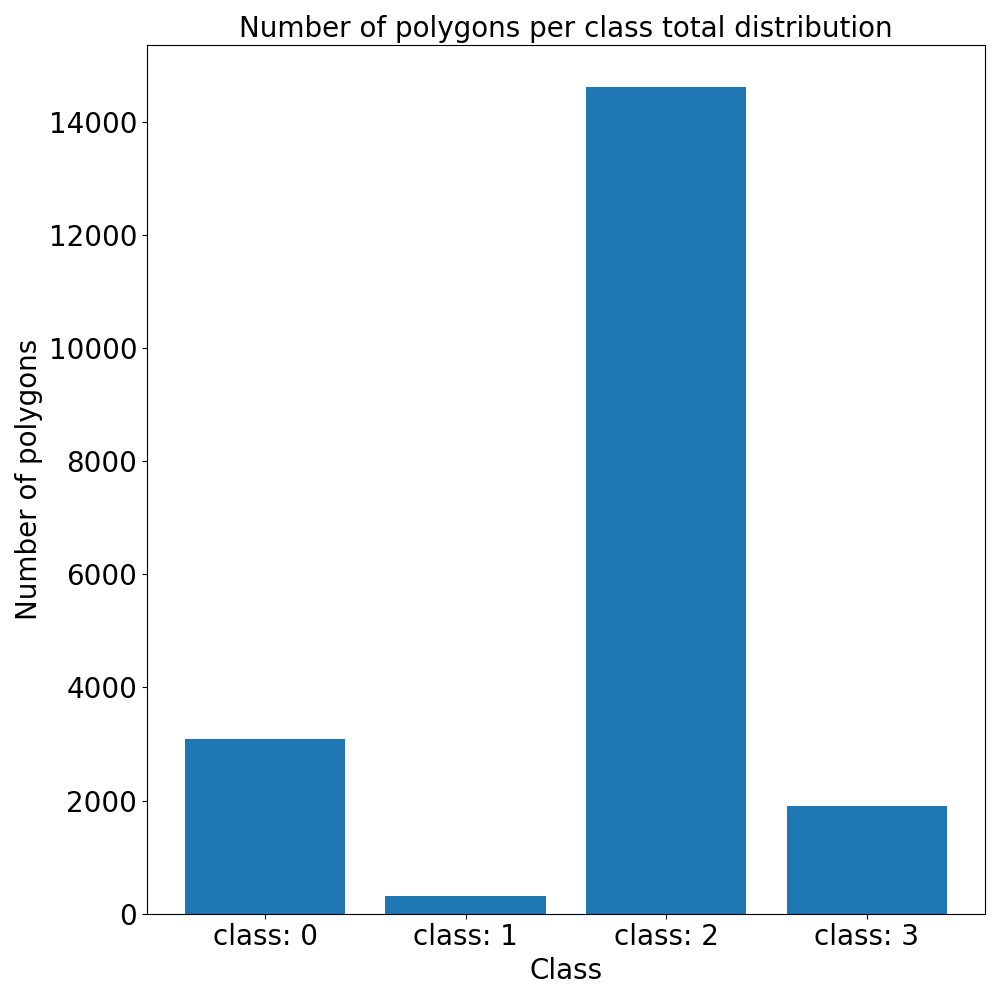
\includegraphics[width=0.45\textwidth]{imgs/Severstal/raw_dataset/n_polygons_per_class_total_histogram.png}
            }  \\
        \end{tabular}
    \end{figure}

Altri parametri interessanti che vanno presi in considerazione riguardano la distribuzione dei poligoni nelle immagini, ovvero la distribuzione del
numero di poligoni in ogni immagine, per avere un'idea della frequenza con cui questi sono presenti. 
Una valutazione è stata fatta anche per la distribuzione dell'area dei poligoni, in quanto ai fini 
della generazione dei difetti sintetici è importante conoscere la quantità di pixel relativa ai difetti a disposizione, consideriamo infatti 
che 10 difetti con area di 100 pixel (1000 pixel) portano con se molta meno informazione di 1 difetto con area di 4000 pixel. 
Le stesse valutazioni sono poi state fatte per ogni classe di difetti, in quanto ogni classe ha una sua specifica distribuzione.

    \begin{figure}[H]
        \centering
        \begin{tabular}{cc}
            % first row
            \subfloat[Distribuzione numero poligoni per immagine.]{
                \label{fig:sd_polygons_per_image_distribution}
                \centering
                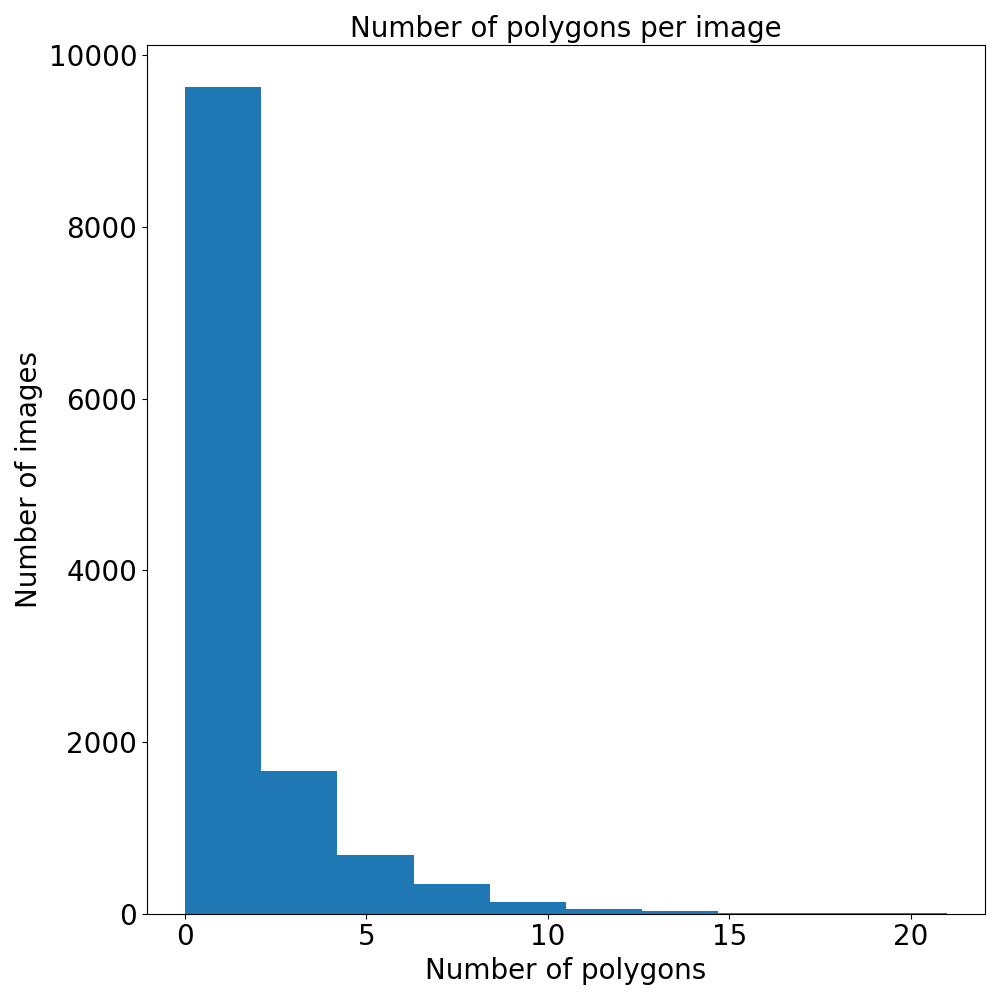
\includegraphics[width=0.45\textwidth]{imgs/Severstal/raw_dataset/n_polygons_per_image_histogram.png}
            }  &
            \subfloat[Distribuzione area poligoni per immagine.]{
                \label{fig:sd_polygons_area_distribution}
                \centering
                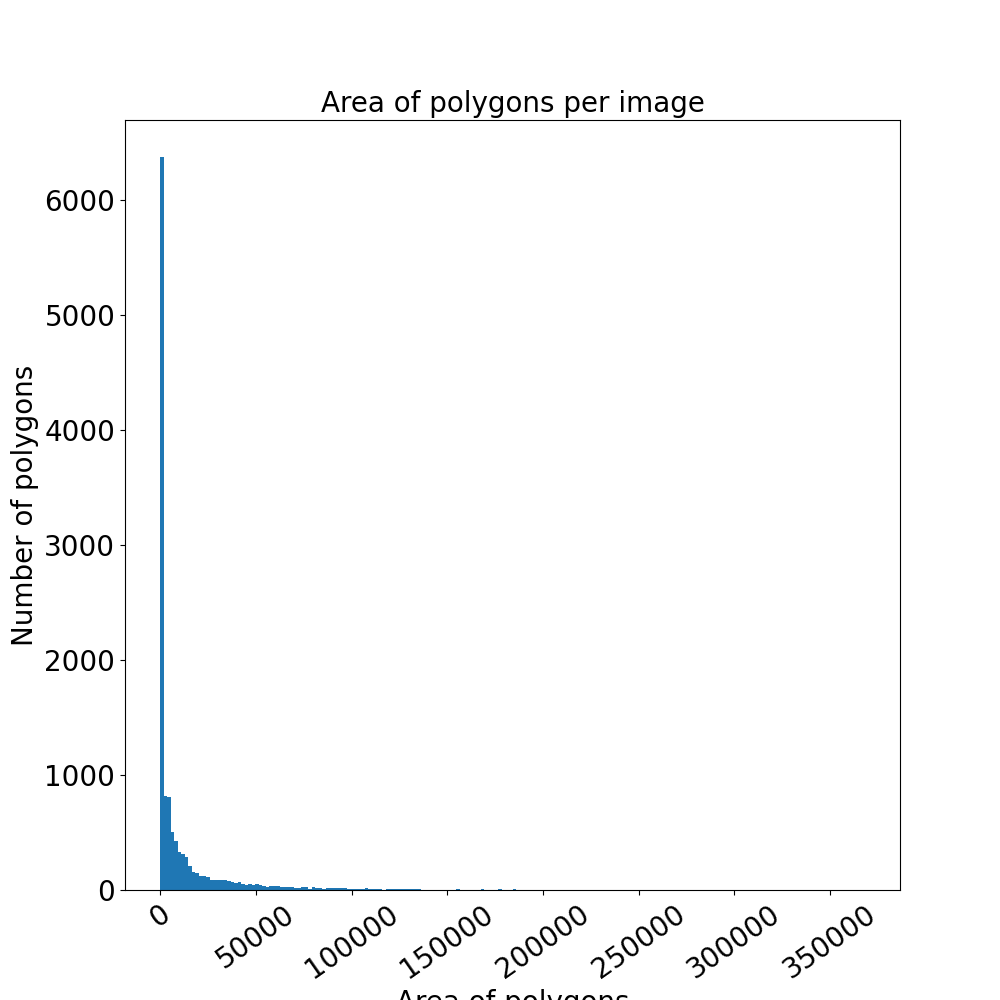
\includegraphics[width=0.45\textwidth]{imgs/Severstal/raw_dataset/area_of_polygons_per_image_histogram.png}
            }  \\ \\

            \subfloat[Distribuzione numero poligoni classe 1 per immagine]{
                \label{fig:sd_polygons_per_image_per_class_distribution_0}
                \centering
                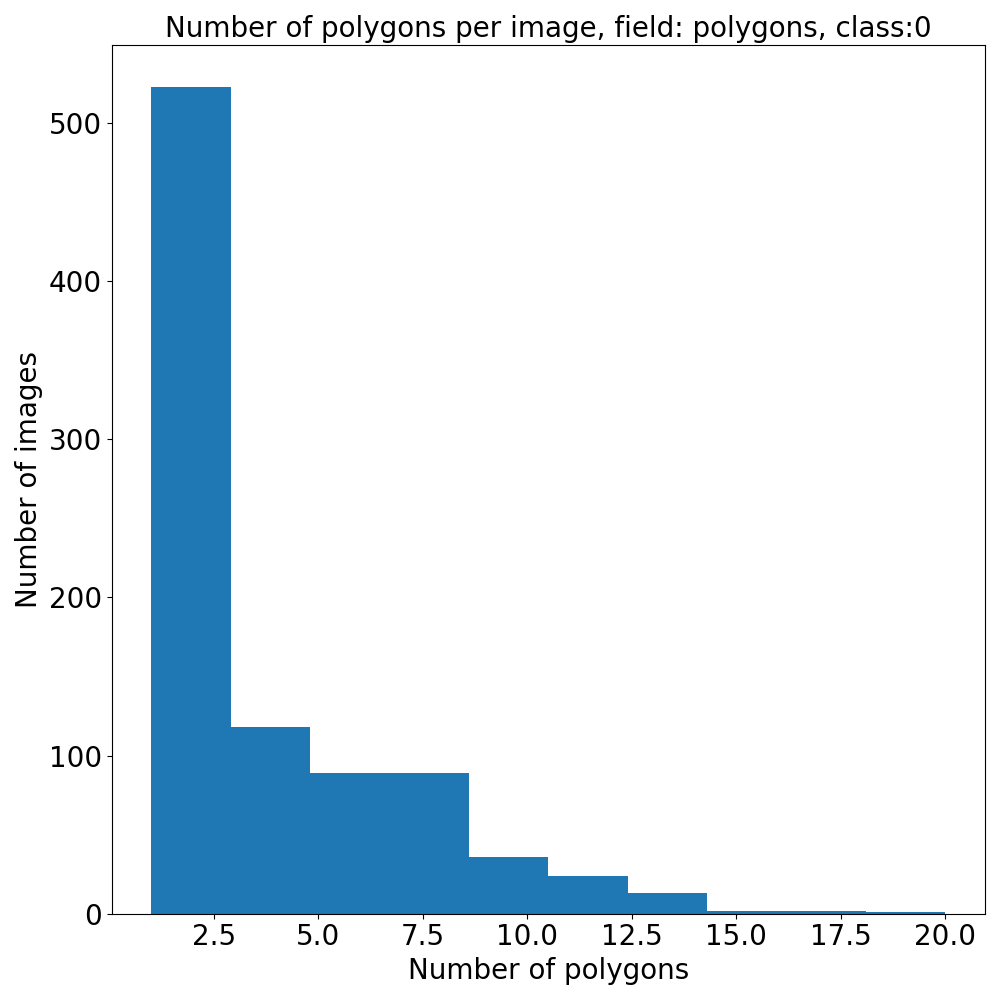
\includegraphics[width=0.45\textwidth]{imgs/Severstal/raw_dataset/n_polygons_per_image_per_class_histogram_polygons_0.png}
            }  &
            \subfloat[Distribuzione numero poligoni classe 2 per immagine]{
                \label{fig:sd_polygons_per_image_per_class_distribution_1}
                \centering
                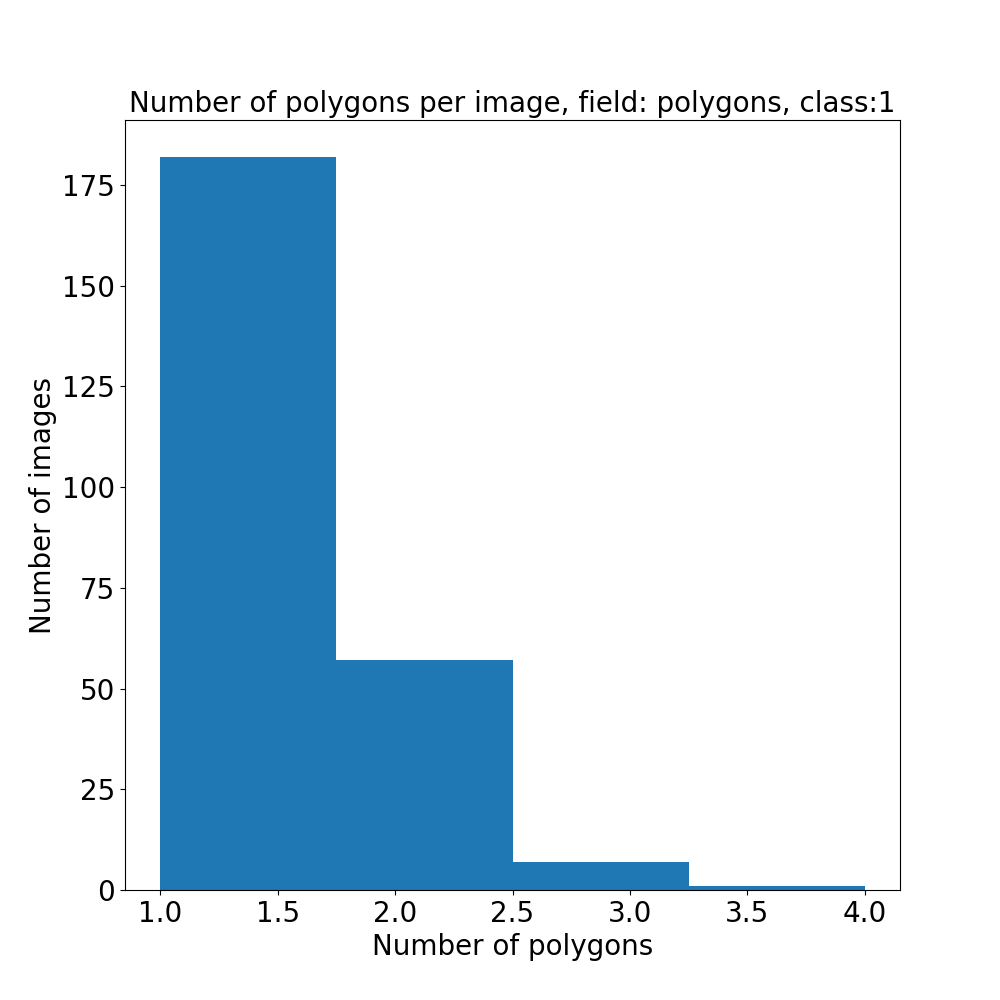
\includegraphics[width=0.45\textwidth]{imgs/Severstal/raw_dataset/n_polygons_per_image_per_class_histogram_polygons_1.png}
            }  \\ \\
            
            \subfloat[Distribuzione numero poligoni classe 3 per immagine]{
                \label{fig:sd_polygons_per_image_per_class_distribution_2}
                \centering
                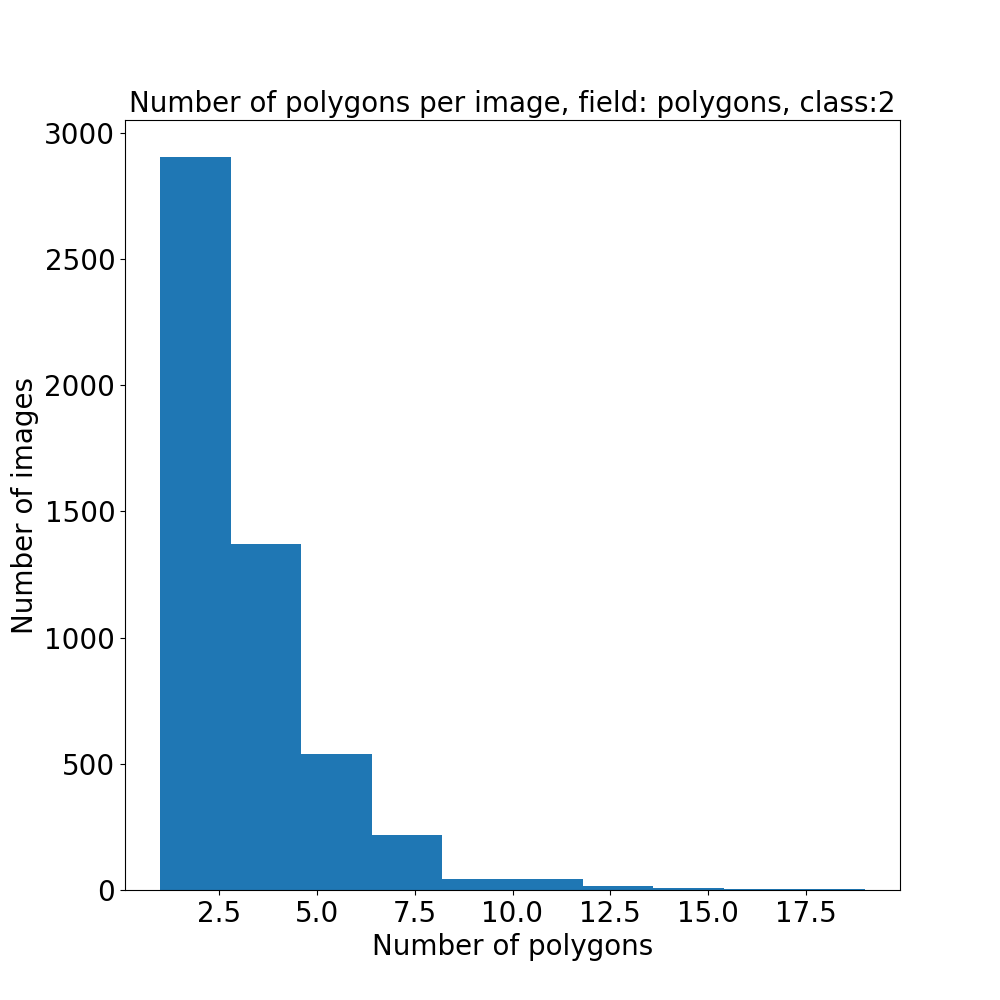
\includegraphics[width=0.45\textwidth]{imgs/Severstal/raw_dataset/n_polygons_per_image_per_class_histogram_polygons_2.png}
            }  &
            \subfloat[Distribuzione numero poligoni classe 4 per immagine]{
                \label{fig:sd_polygons_per_image_per_class_distribution_3}
                \centering
                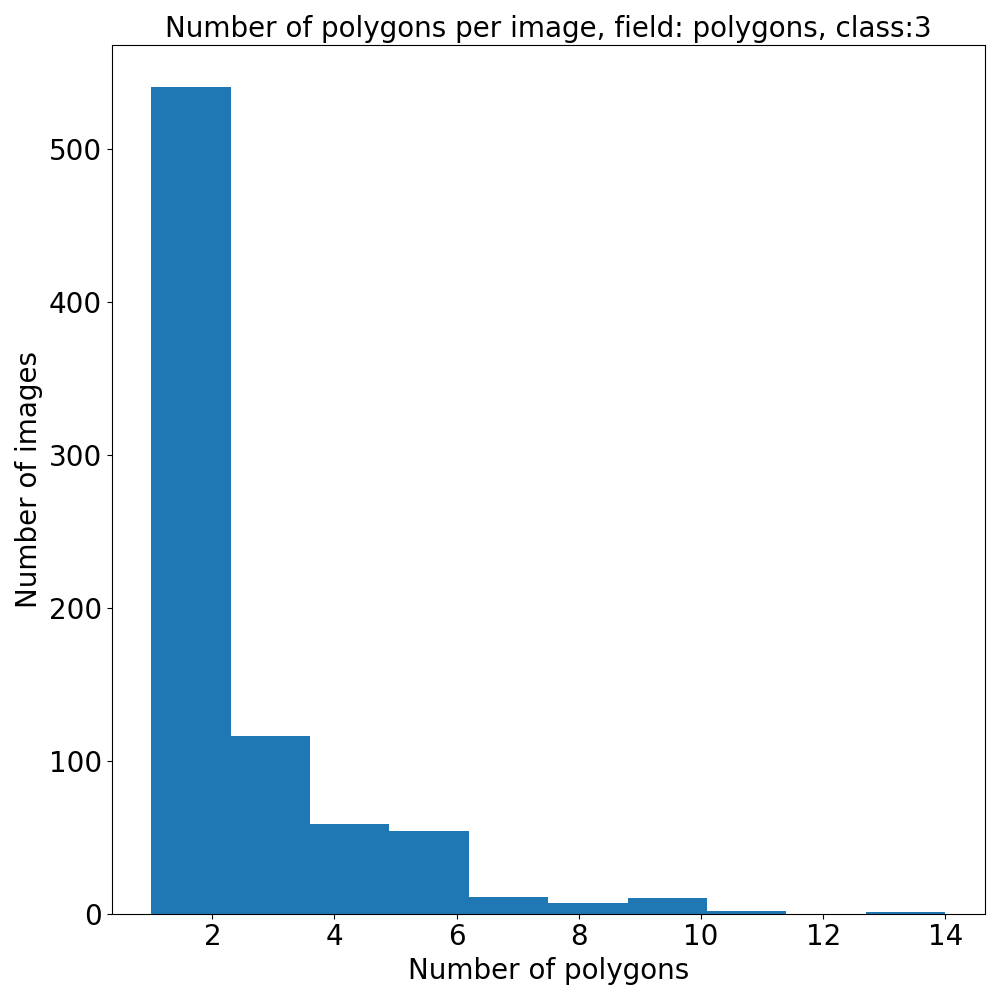
\includegraphics[width=0.45\textwidth]{imgs/Severstal/raw_dataset/n_polygons_per_image_per_class_histogram_polygons_3.png}
            }  \\
        \end{tabular}
    \end{figure}

    \begin{figure}[H]
        \centering
        \begin{tabular}{cc}
            % first row 
            \subfloat[Distribuzione area poligoni classe 1.]{
                \label{fig:sd_polygons_area_distribution_0}
                \centering
                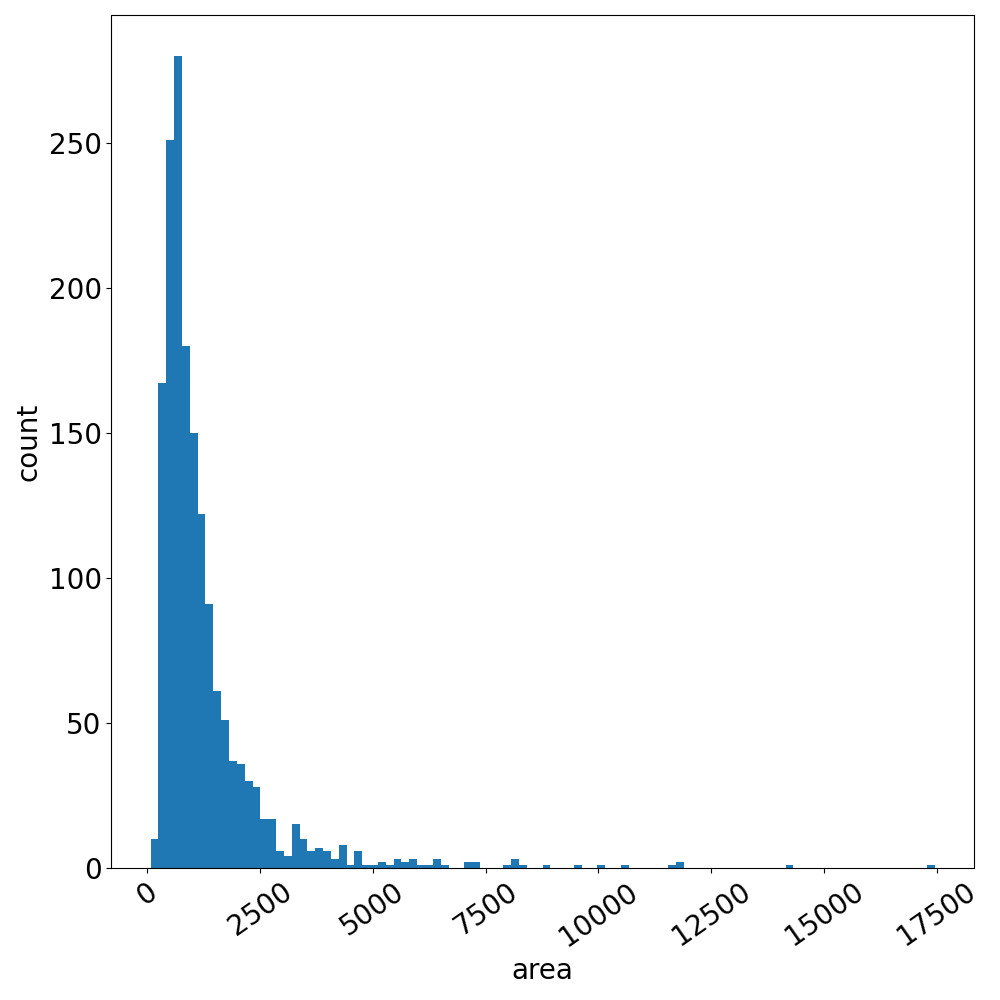
\includegraphics[width=0.45\textwidth]{imgs/Severstal/crop_defects_distr/class_0/area_hist.png}
            }  &
            \subfloat[Distribuzione aspect-ratio poligoni classe 1.]{
                \label{fig:sd_polygons_aspect_ratio_distribution_0}
                \centering
                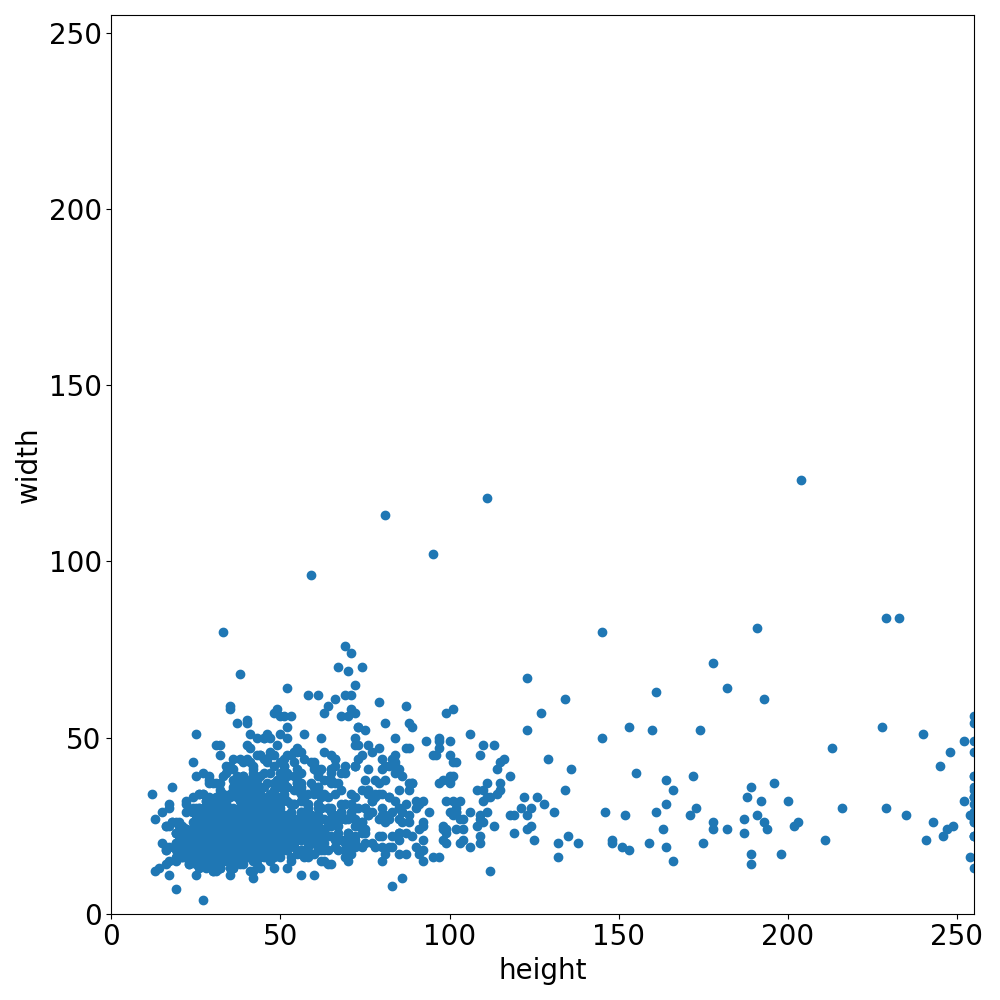
\includegraphics[width=0.45\textwidth]{imgs/Severstal/crop_defects_distr/class_0/shape_scatter.png}
            } \\
        \end{tabular}
    \end{figure}

    \begin{figure}[H]
        \centering
        \begin{tabular}{cc}
            \subfloat[Distribuzione area poligoni classe 2.]{
                \label{fig:sd_polygons_area_distribution_1}
                \centering
                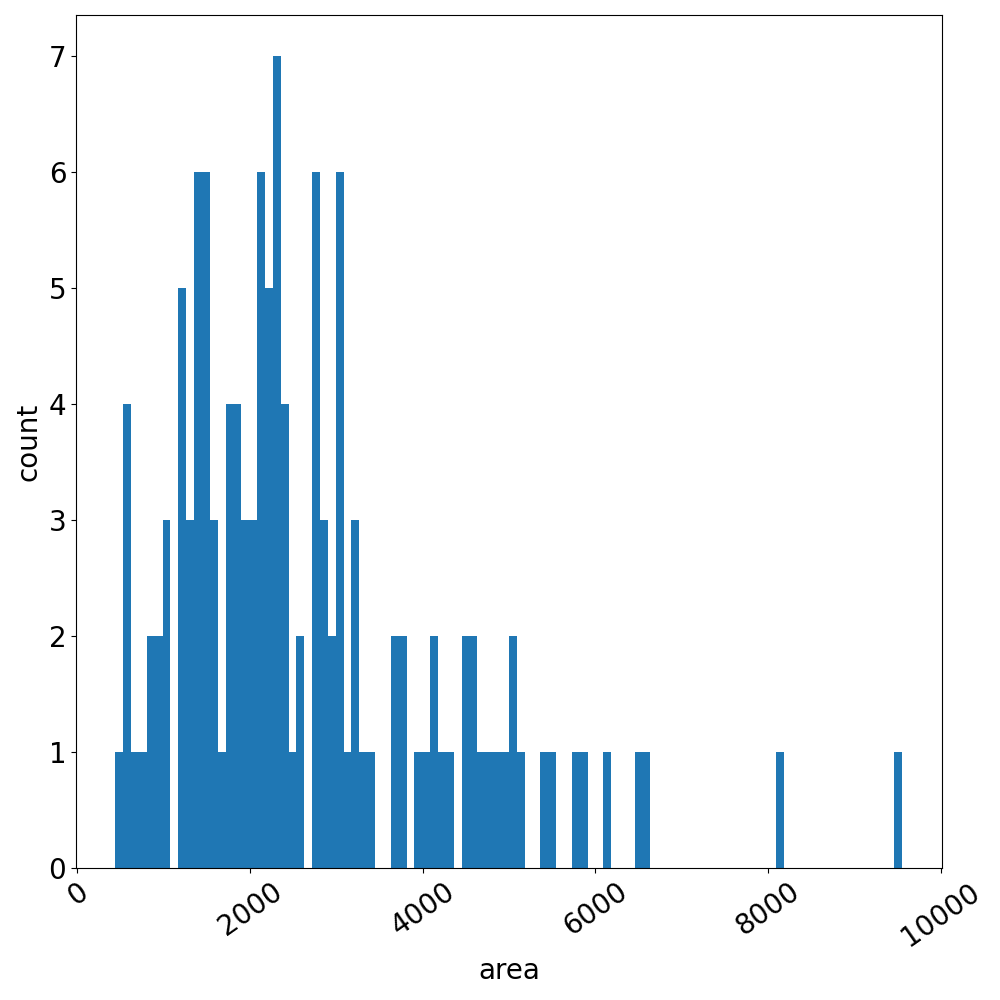
\includegraphics[width=0.45\textwidth]{imgs/Severstal/crop_defects_distr/class_1/area_hist.png}
            }  &
            
            \subfloat[Distribuzione aspect-ratio poligoni classe 2.]{
                \label{fig:sd_polygons_aspect_ratio_distribution_1}
                \centering
                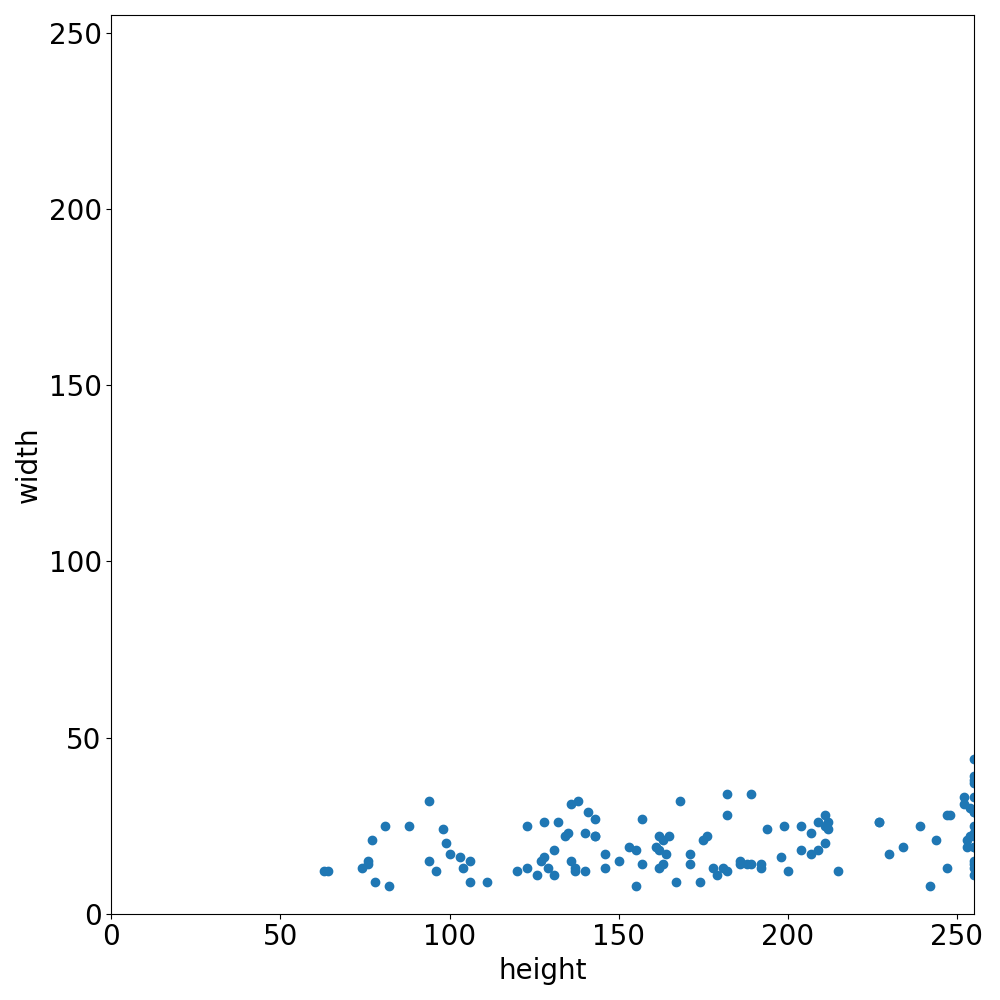
\includegraphics[width=0.45\textwidth]{imgs/Severstal/crop_defects_distr/class_1/shape_scatter.png}
            } \\
        \end{tabular}
    \end{figure}
    
    \begin{figure}[H]
        \centering
        \begin{tabular}{cc}
            \subfloat[Distribuzione area poligoni classe 3.]{
                \label{fig:sd_polygons_area_distribution_2}
                \centering
                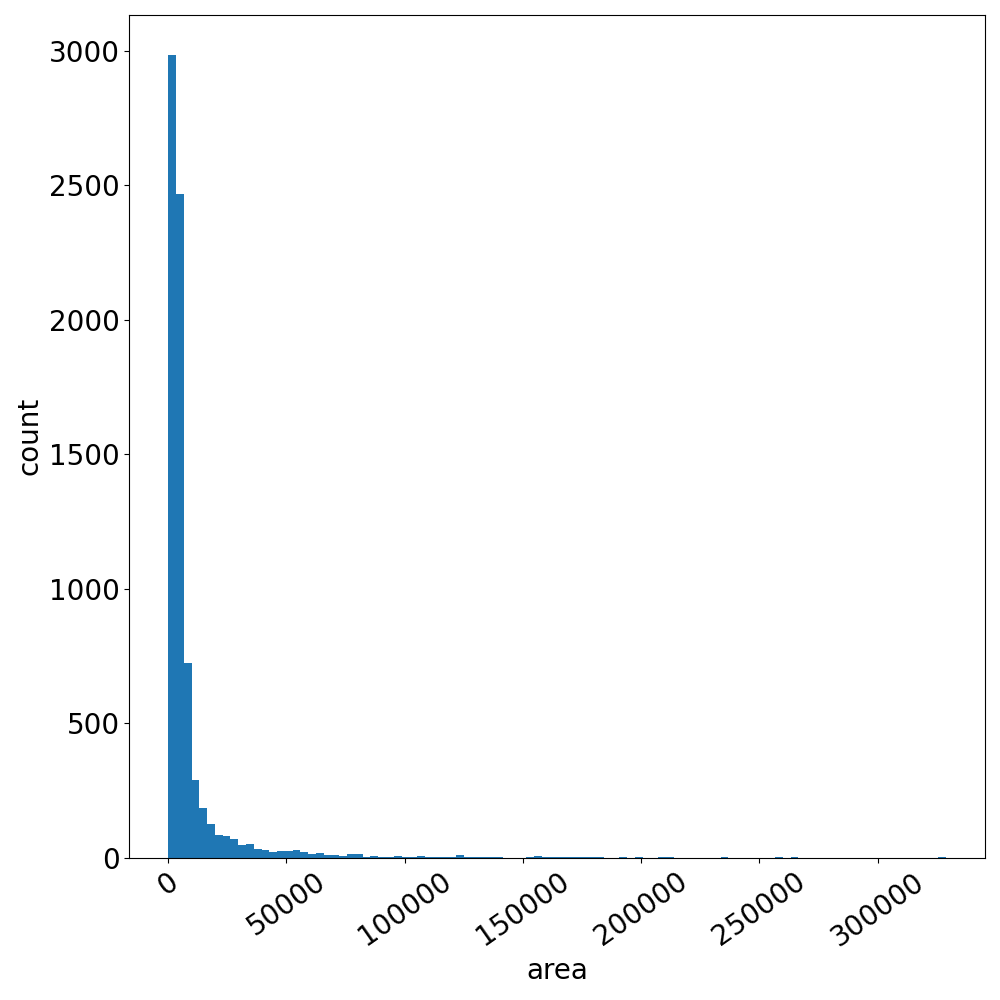
\includegraphics[width=0.45\textwidth]{imgs/Severstal/crop_defects_distr/class_2/area_hist.png}
            }  &
            \subfloat[Distribuzione aspect-ratio poligoni classe 3.]{
                \label{fig:sd_polygons_aspect_ratio_distribution_2}
                \centering
                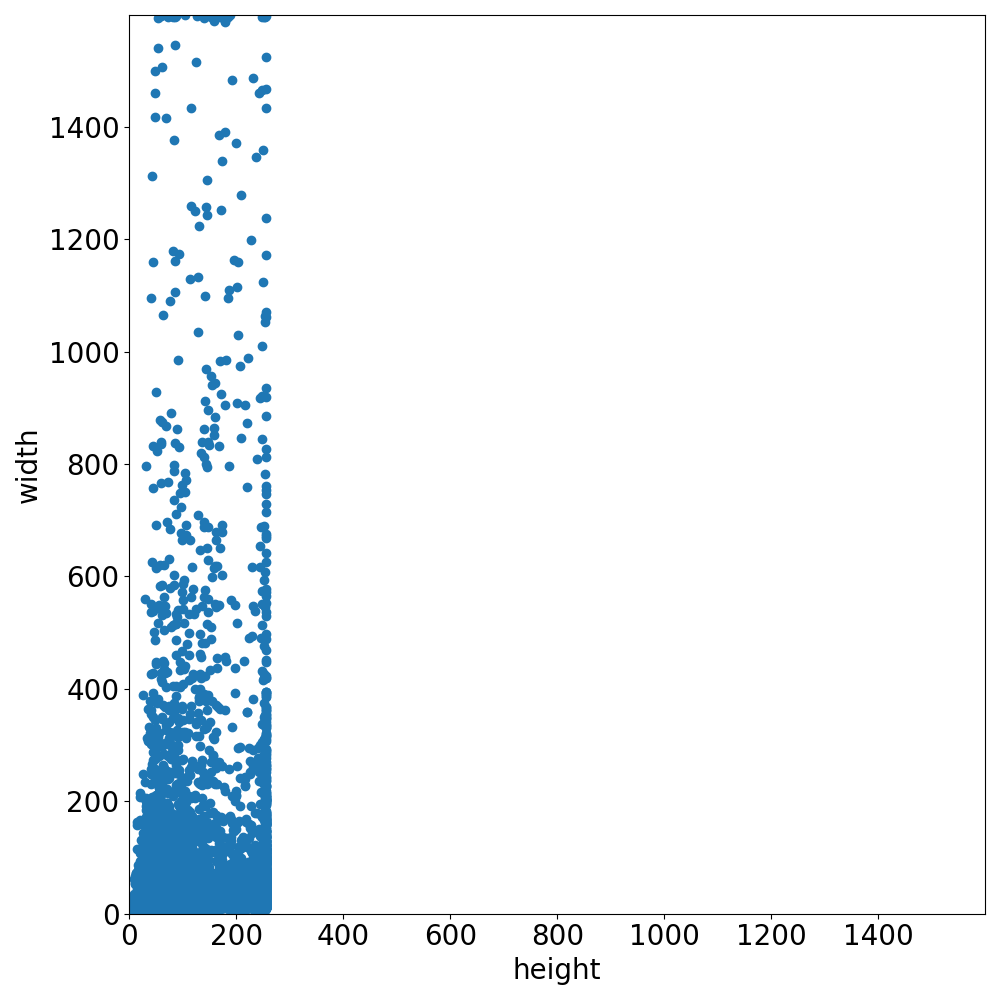
\includegraphics[width=0.45\textwidth]{imgs/Severstal/crop_defects_distr/class_2/shape_scatter.png}
            } \\
        \end{tabular}
    \end{figure}
    
    \begin{figure}[H]
        \centering
        \begin{tabular}{cc}
            \subfloat[Distribuzione area poligoni classe 4.]{
                \label{fig:sd_polygons_area_distribution_3}
                \centering
                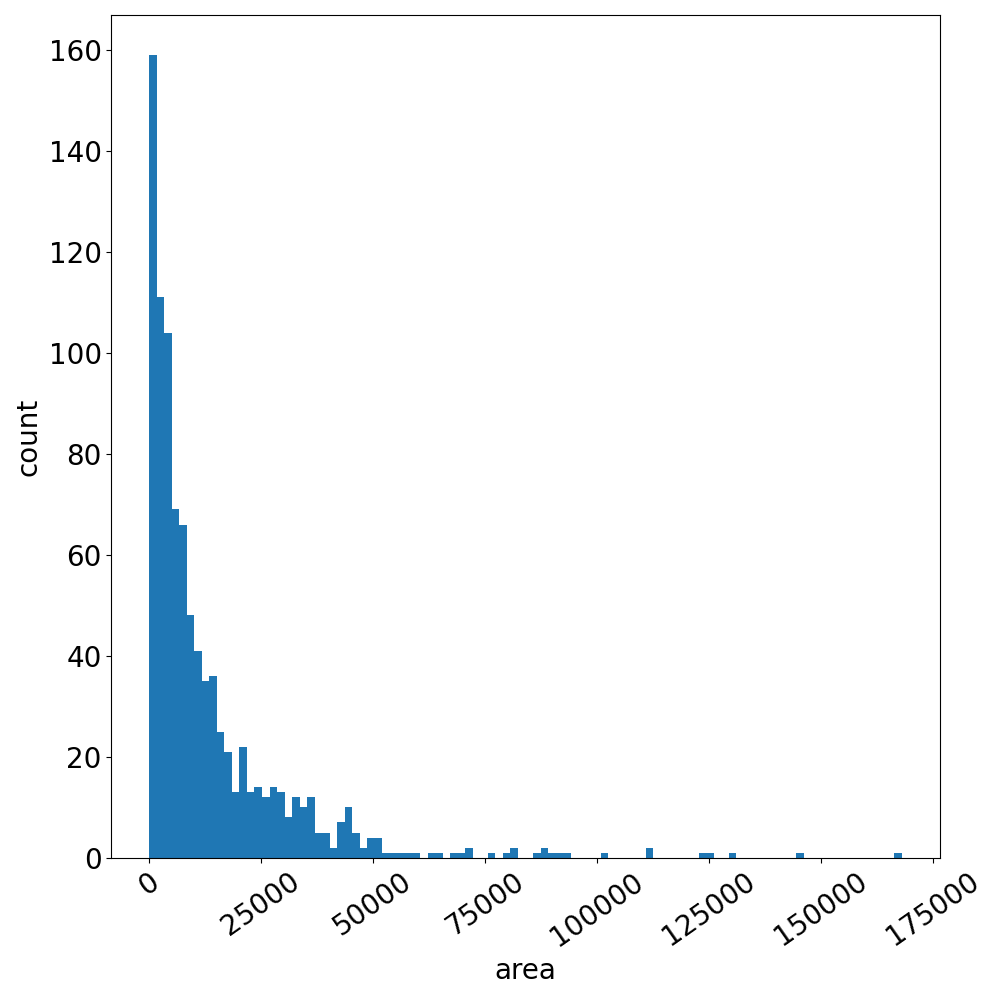
\includegraphics[width=0.45\textwidth]{imgs/Severstal/crop_defects_distr/class_3/area_hist.png}
            }  &
            \subfloat[Distribuzione aspect-ratio poligoni classe 4.]{
                \label{fig:sd_polygons_aspect_ratio_distribution_3}
                \centering
                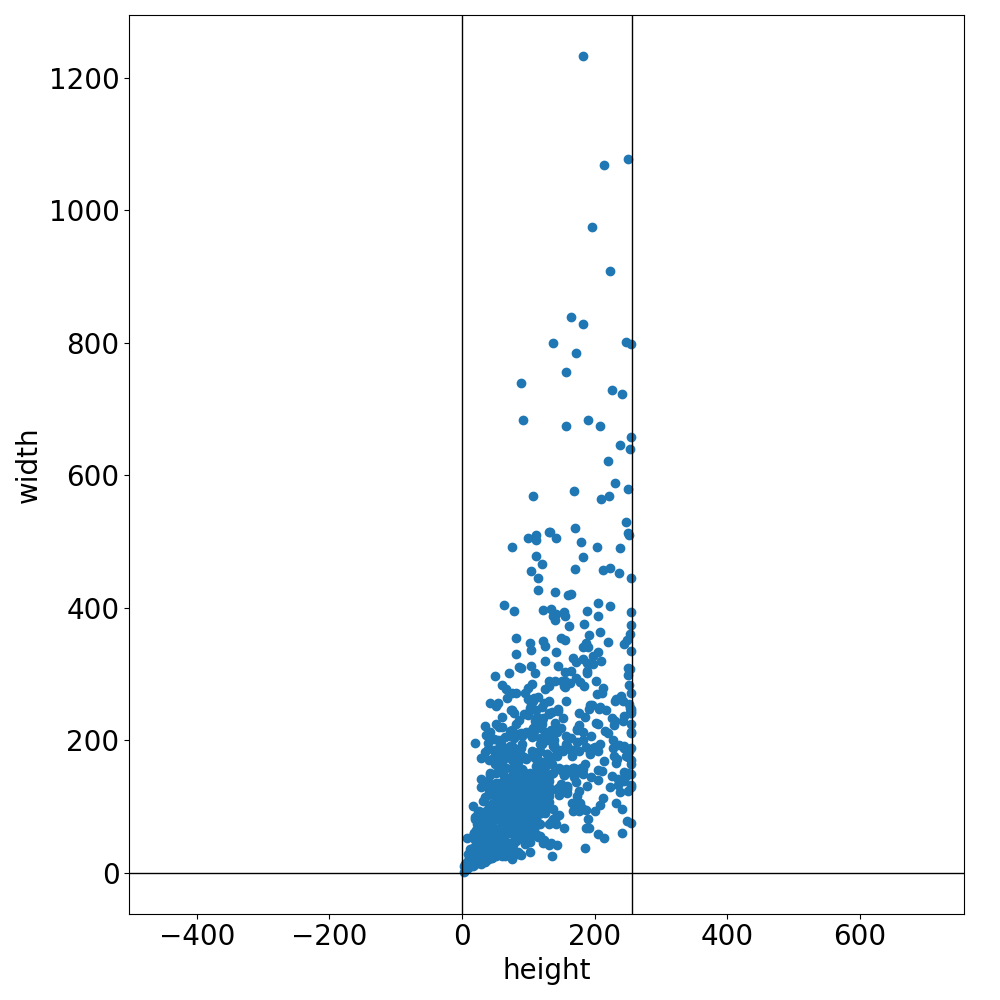
\includegraphics[width=0.45\textwidth]{imgs/Severstal/crop_defects_distr/class_3/shape_scatter.png}
            } \\
        \end{tabular}
    \end{figure}

Vediamo di seguito alcuni esempi di difetti estratti dal dataset tramite crop, appartenenti alle quattro classi. 
Con il dataset non vengono fornite informazioni riguardo alle caratteristiche delle 4 classi ma è possibile dedurre 
alcune informazioni analizzando le immagini e le distribuzioni mostrate.
Si noti che gli esempi mostrati di seguito in alcuni casi sono stati ridimensionati o ruotati per una migliore illustrazione.

\begin{figure}[H]
    \centering 
    \begin{tabular}{cc}
        \subfloat[Esempi di difetti classe 1.]{
            \label{fig:sd_class_0}
            \centering
            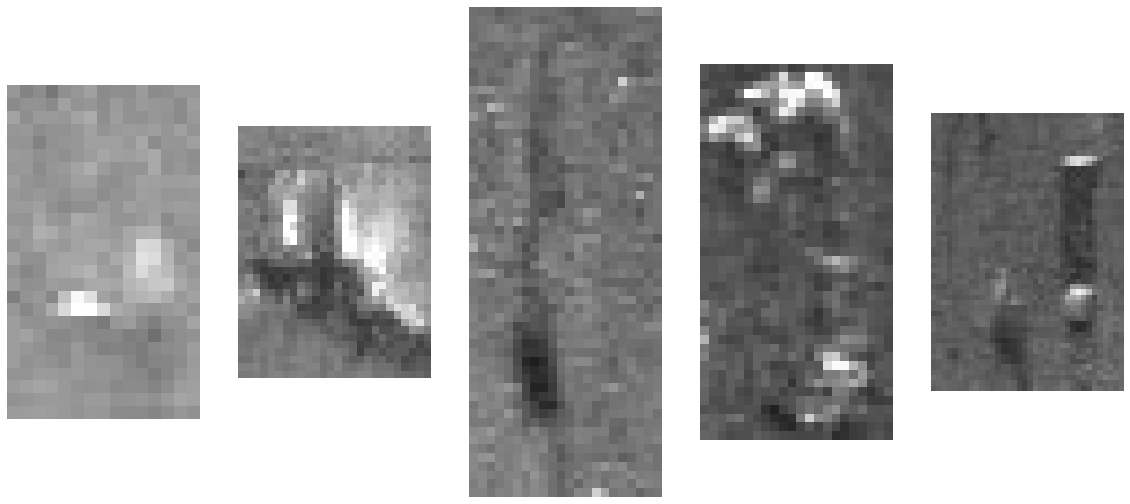
\includegraphics[width=0.45\textwidth]{imgs/Severstal/defect_samples/samples_class_0.png}
        }  &
        \subfloat[Esempi di difetti classe 2.]{
            \label{fig:sd_class_1}
            \centering
            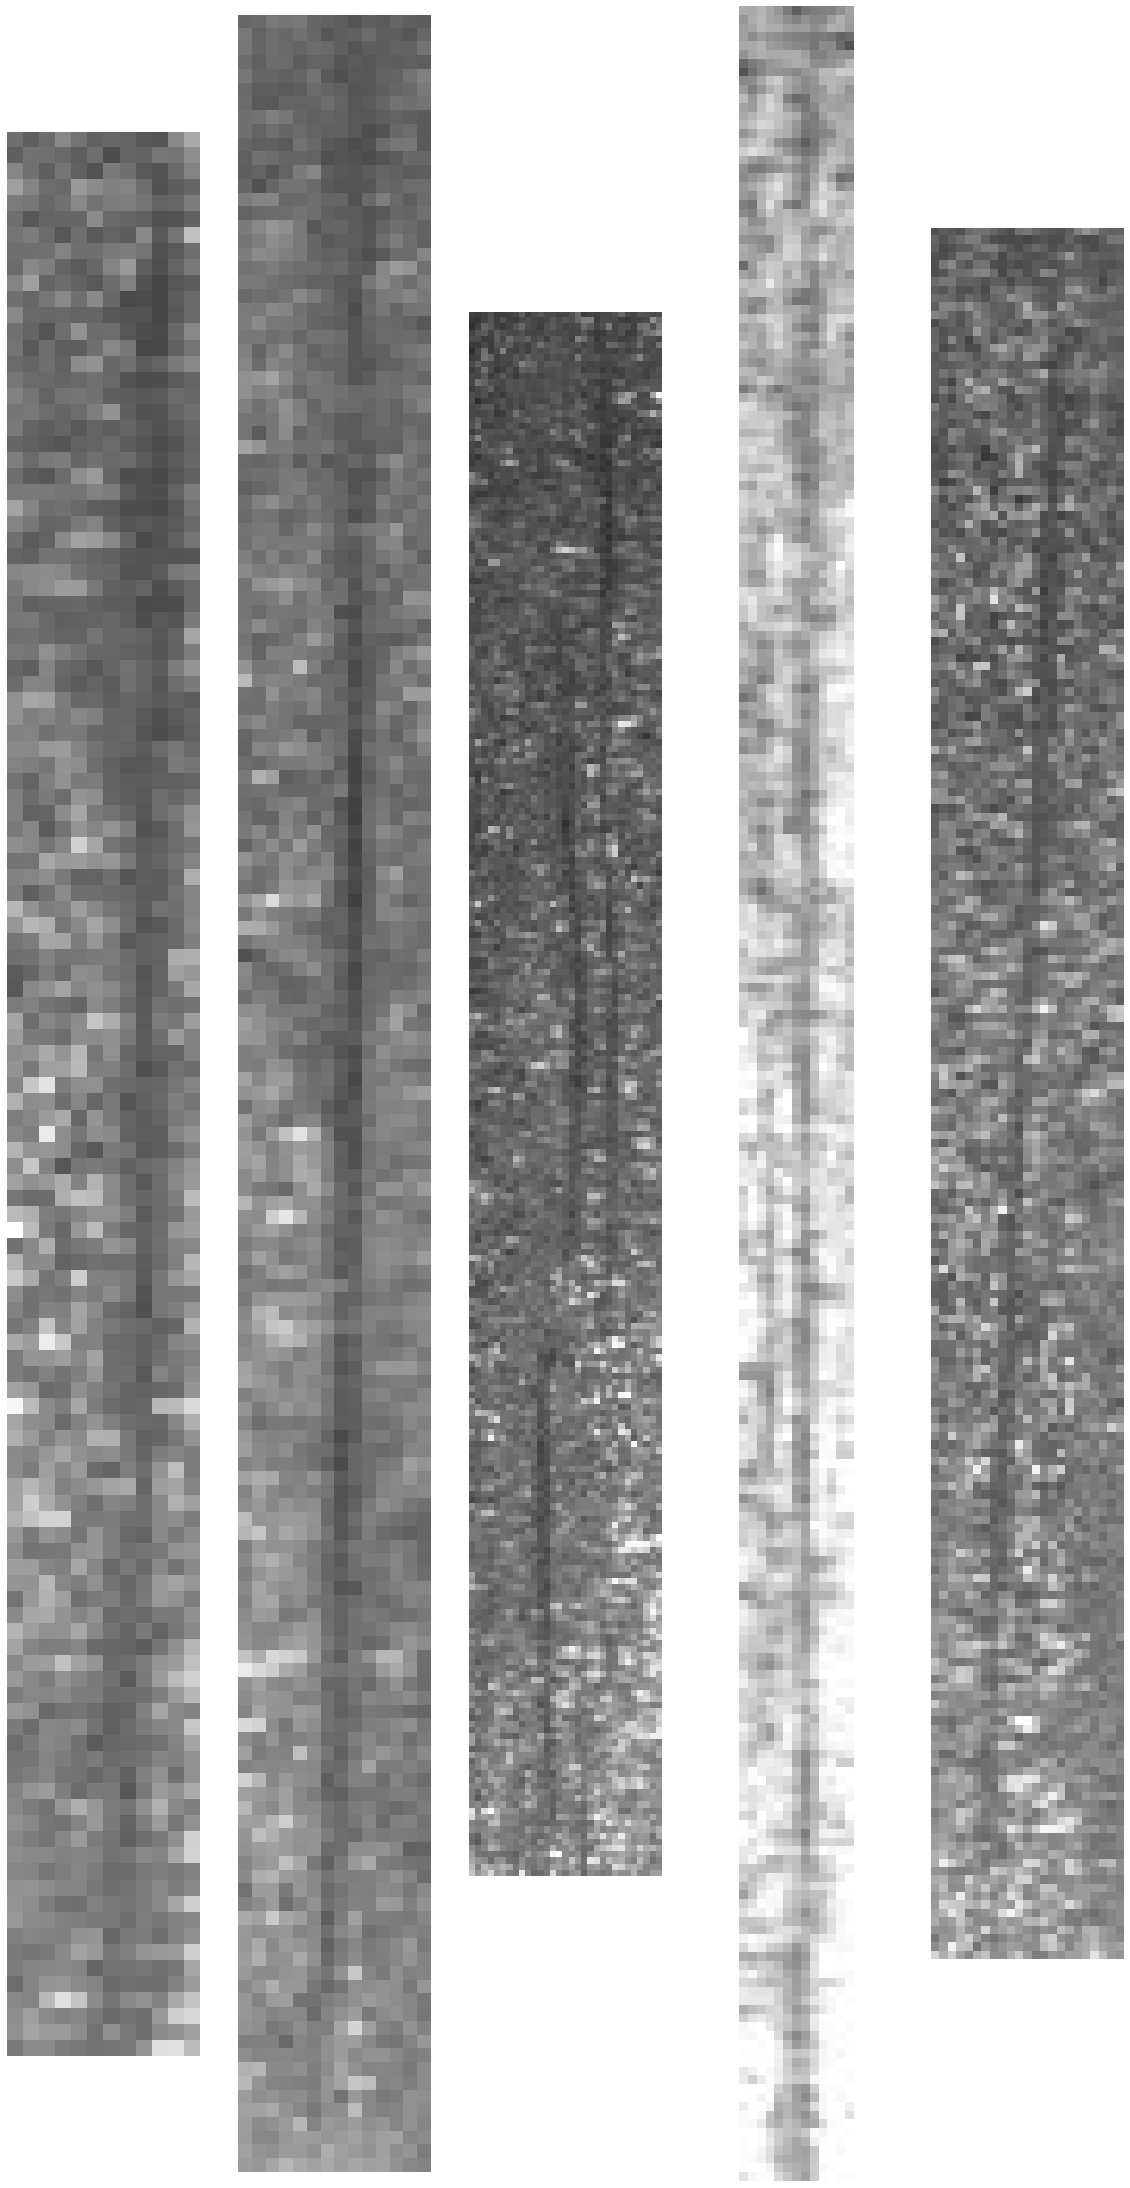
\includegraphics[width=0.2\textwidth]{imgs/Severstal/defect_samples/samples_class_1.png}
        }  \\
        \subfloat[Esempi di difetti classe 3.]{
            \label{fig:sd_class_2}
            \centering
            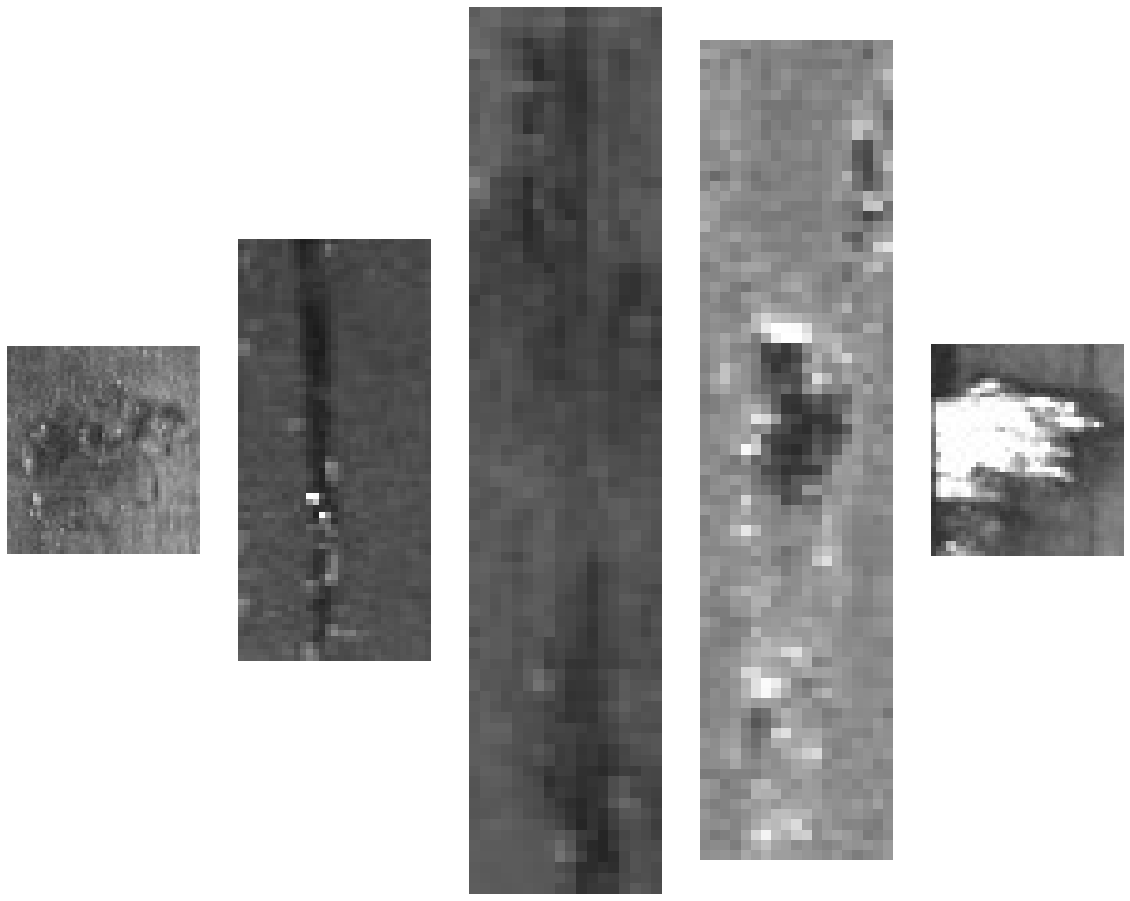
\includegraphics[width=0.45\textwidth]{imgs/Severstal/defect_samples/samples_class_2.png}
        } &
        \subfloat[Esempi di difetti classe 4.]{
            \label{fig:sd_class_3}
            \centering
            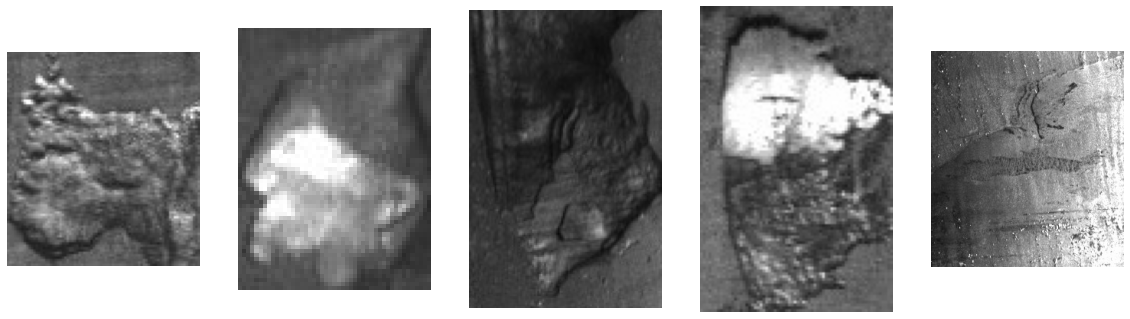
\includegraphics[width=0.45\textwidth]{imgs/Severstal/defect_samples/samples_class_3.png}
        } \\
    \end{tabular}
\end{figure}






\section{Librerie e Framework\ok}
\begin{comment}
    In this section i can talk about python and the most important libraries i used
    in the project like pytorch and OpenCv, and why i used them.
\end{comment}
In questo progetto è stato utilizzato il linguaggio python che ad oggi è uno dei linguaggi più utilizzati per il machine learning e l'intelligenza artificiale,
data la sua semplicità e la sua versatilità, per non parlare della vasta scelta di librerie che offre.
Nonostante python sia un linguaggio interpretato, è possibile utilizzarlo per applicazioni che richiedono un alto livello di performance,
in quanto le librerie che si occupano di effettuare le operazioni più pesanti, sono scritte in C/C++, e vengono 
utilizzate tramite python bindings, che permettono di utilizzare le librerie scritte in C/C++ come se fossero state scritte in python,
è questo il caso di librerie come Numpy, OpenCv, Pytorch, ecc.

\subsection{Numpy\ok}
Una delle librerie più importanti per python è Numpy, che permette di lavorare con array multidimensionali, e di effettuare operazioni su di essi 
in modo efficiente con un'interfaccia semplice e intuitiva. Questa libreria benche non sia integrata in python, è una delle librerie più utilizzate
ed è uno standard de facto per il calcolo scientifico per svariate librerie per python.

\subsection{OpenCV\ok}
OpenCV è una libreria open source per il computer vision, scritta in C++, ma utilizzabile anche in python tramite python bindings.
Ad oggi è una delle librerie più utilizzate per l'elaborazione di immagini e video, in quanto offre un'ampia gamma di funzionalità.
In questo progetto è stata utilizzata per effettuare diverse operazioni di pre-elaborazione del dataset, e per lo script demo di inferenza.

\subsection{Pytorch\ok}
Pytorch è un framework open source per il deep learning, sviluppato da Facebook, che permette di effettuare operazioni su tensori in modo efficiente
sfruttando le GPU, e di effettuare automaticamente il backpropagation, rendendo l'operazione di definire una rete neurale e addestrarla
molto semplice e veloce.

\subsection{Distributed data parallel}
Distributed data parallel non è una libreria a se stante ma un modulo integrato nel framework Pytorch,
che permette di scalare il training di un modello neurale su più GPU in un singolo nodo, o su più nodi.
DDP parallelizza il training generando un processo separato per ogni GPU, ognuno presenta
una copia identica del modello, durante il training la retropropagazione dell'errore innesca un \textit{hook} che effettua la 
sincronizzazione dei gradienti mediante delle primitive di sincronizzazione tra i processi, in tal modo 
si ottiene un unico gradiente aggiornato per tutte le istanze.


\begin{comment}
    Aggiungi un ulteriore strumento degno di nota
\end{comment}

\section{Google cloud compute instance\ok}
L'addestramento del modello neurale è stato effettuato mediante l'utilizzo dei servizi di Google Cloud Platform, 
in particolare è stata utilizzata una macchina virtuale \textbf{n1-standard-8} con le seguenti caratteristiche:

\begin{itemize}
    \item \textbf{Sistema Operativo:} Ubuntu 18.04
    \item \textbf{CPU:} 8 vCPU
    \item \textbf{GPU:} 2x Nvidia Tesla T4 (16 GB)
    \item \textbf{RAM:} 32 GB 
\end{itemize}

Questa tipologia di macchina virtuale è una delle consigliate per l'addestramento di modelli di deep learning, in quanto permette di utilizzare
le GPU T4 di Nvidia, le quali ad oggi costituiscono un ottimo compromesso tra costo e performance. Infatti l'affitto di una macchina
virtuale con queste caratteristiche, con ben 2 Tesla T4, per un mese ha un costo di circa 500 euro, mentre una macchina virtuale con una sola GPU 
come una V100 o una A100 può superare tranquillamente i 3000€.

Questa configurazione non garantisce le stesse performance delle controparti di fascia alta ma comunque consentono di avere a disposizione
una potenza di calcolo discreta e un quantitativo di memoria di ben 32 GB di memoria GDDR6, che è più che sufficiente per l'addestramento di modelli
neurali di modeste dimensioni se pur con dimensioni di batch ridotte.

\section{Repository del progetto}
Il codice sorgente del progetto è disponibile su GitHub al seguente indirizzo: 

\url{https://github.com/MassimilianoBiancucci/COIGAN-controllable-object-inpainting}

Nel repository è presente il codice effettivo per eseguire un training, il codice per effettuare la preparazione del
dataset, il quale necessita di un formato particolare, e lo script per effettuare una valutazione interattiva del modello.
Tutti i passaggi necessari per preparare l'ambiente, e sistemare i file di configurazione sono descritti nel file README.md.

